% !TEX root = slides.tex
%==============================================================================
\begin{frame}[t]
\label{merr7a}

\frametitle{Model Error -- Surrogate and Prediction}
\vspace*{-0.2cm}

% \centerline{\hspace*{9cm}$\qquad$
% \begin{tikzpicture} \node [rounded corners,fill=blue!20] {
% $g_i \approx f_i(\lambda(\zeta;\alpha))$
% };
% \end{tikzpicture}
% }

% %\vspace*{0.7cm}

\centerline{
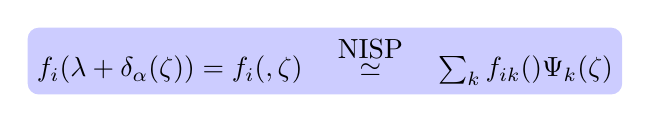
\begin{tikzpicture} \node [rounded corners,fill=blue!20] {
$f_i(\lambda+\delta_\alpha(\zeta))=f_i(\tlam,\zeta) \quad\stackrel{\textrm{NISP}}{\simeq} \quad\sum_k f_{ik}(\tlam) \Psi_k(\zeta)$
};
\end{tikzpicture}
}

\bi
\setlength{\itemsep}{3mm}
\setlength{\itemindent}{-4.4mm}
\item NISP is employed both for likelihood computation and for posterior/pushed-forward predictions in general
\item In practice, $f_i(\cdot)$ is replaced by a pre-constructed polynomial surrogate
\item Note: NISP with finite truncation is exact, \\
if one truncates NISP at the same order as the surrogate of $f_i(\cdot)$
\item Posterior predictive moments
%\vspace*{-0.1cm}
\[
\mu_i=\EE_{\tlam}\left[\mu_i(\tlam)\right]
\]
\[
 \sigma_i^{2}=\underbrace{\EE_{\tlam}\left[\sigma_i^2(\tlam)\right]}_{\textrm{Model error}} +\underbrace{\VV_{\tlam}\left[\mu_i(\tlam)\right]}_{\textrm{Posterior uncertainty}}  +\underbrace{(\sigma^{LOO}_i)^2}_{\textrm{Surrogate error}}
\]
%\hspace*{3.54cm}$\zeta$\hspace*{2cm}$\alpha$\hspace*{2cm}$\eta$
% \item Added surrogate error leave-one-out (LOO) estimate $\left(\sigma_i^{LOO}\right)^2$ to the overall prediction variance

\ei

\end{frame}
%==================================================================================
